\documentclass{math}

\usepackage{tikz}

\title{University Physics 2}
\author{Alvin Lin}
\date{January 2018 - May 2018}

\begin{document}

\maketitle

\section*{Electric Fields}
We know positive charges feel repulsive forces from other positive charges. If
we take a test charge and place it near an object of interest, how it would
experience a force is the direction of the electric field, also known as the
E-field. We define it as:
\[ \vec{E} = \frac{\vec{F_{\circ}}}{q_{\circ}} \]
where \( \vec{F_{\circ}} \) is the force on the test charge, \( q_{\circ} \)
is the test charge, and \( \vec{E} \) is the electric field from some charge
distribution. Usually, we will represent this in the form:
\[ \vec{F} = q\vec{E} \]
This allows us to calculate the force \( \vec{F} \) for some charge \( q \)
exerted by an external electric field \( \vec{E} \). For a point charge, we
calculate the field with:
\[ \vec{E_{pc}} = \frac{Kq\hat{r}}{r^2} \]
This is the same as Coulomb's Law but is measured in Newtons per Coulomb. This
is due to the fact that there is no second charge from the observation charge.
The field lines point away from positive charges and towards negative charges.
\begin{center}
  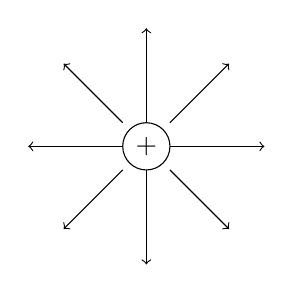
\begin{tikzpicture}[scale=1.5]
    \draw (0,0) circle (0.2cm) node {+};
    \draw[->] (0.2,0) -- (1,0);
    \draw[->] (0.2,0.2) -- (0.7,0.7);
    \draw[->] (0,0.2) -- (0,1);
    \draw[->] (-0.2,0.2) -- (-0.7,0.7);
    \draw[->] (-0.2,0) -- (-1,0);
    \draw[->] (-0.2,-0.2) -- (-0.7,-0.7);
    \draw[->] (0,-0.2) -- (0,-1);
    \draw[->] (0.2,-0.2) -- (0.7,-0.7);
  \end{tikzpicture}
  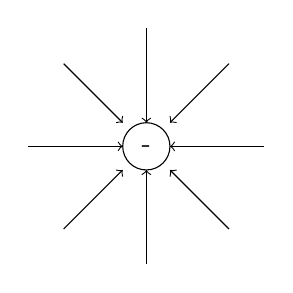
\begin{tikzpicture}[scale=1.5]
    \draw (0,0) circle (0.2cm) node {-};
    \draw[<-] (0.2,0) -- (1,0);
    \draw[<-] (0.2,0.2) -- (0.7,0.7);
    \draw[<-] (0,0.2) -- (0,1);
    \draw[<-] (-0.2,0.2) -- (-0.7,0.7);
    \draw[<-] (-0.2,0) -- (-1,0);
    \draw[<-] (-0.2,-0.2) -- (-0.7,-0.7);
    \draw[<-] (0,-0.2) -- (0,-1);
    \draw[<-] (0.2,-0.2) -- (0.7,-0.7);
  \end{tikzpicture}
\end{center}

\subsection*{Electric Dipoles: Off-Axis Field}
\begin{center}
  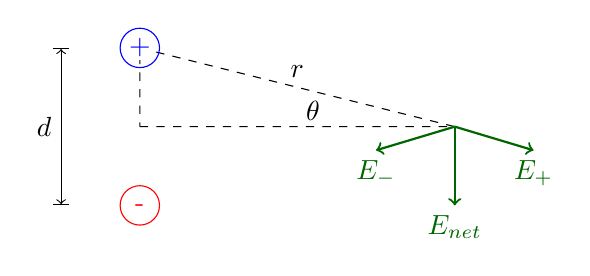
\begin{tikzpicture}
    \draw[|<->|] (-1,1) -- (-1,-1) node[pos=0.5,left] {\( d \)};
    \draw[dashed] (0,0) -- (4,0) -- node[pos=0.5,above] {\( r \)} (0,1) --
      cycle;
    \node at (2.2,0.2) {\( \theta \)};
    \draw[blue] (0,1) circle (0.25cm) node[fill=white,inner sep=0.04cm] {+};
    \draw[red] (0,-1) circle (0.25cm) node[fill=white,inner sep=0.04cm] {-};
    \draw[->,thick,black!60!green] (4,0) -- (3,-0.3) node[below] {\( E_{-} \)};
    \draw[->,thick,black!60!green] (4,0) -- (5,-0.3) node[below] {\( E_{+} \)};
    \draw[->,thick,black!60!green] (4,0) -- (4,-1) node[below] {\( E_{net} \)};
  \end{tikzpicture}
\end{center}
The x-components of the fields cancel.
\begin{align*}
  E_{+} &= \frac{kq}{r^2} \\
  E_{+,y} &= E_{+}\sin\theta = \frac{kq\sin\theta}{r^2}
\end{align*}
In the case where \( \frac{d}{x} << 1 \):
\[ \left(\frac{d}{x}\right)^2 \approx 0 \]
\begin{align*}
  \sin\theta &= \frac{\frac{d}{2}}{r} \quad r = \sqrt{x^2+(\frac{d}{2})^2} \\
  E_{+,y} &= \frac{kq\sin\theta}{r^2}
    = \frac{kq}{r^2}\frac{\frac{d}{2}}{r}
    = \frac{1}{2}\frac{kqd}{r^3} \\
  &= \frac{1}{2}\frac{kqd}{\bigg(\sqrt{x^2+\frac{d^2}{4}}\bigg)^3} \\
  &= \frac{1}{2}kqd\bigg[x^2+\frac{d^2}{4}\bigg]^{-\frac{3}{2}} \\
  &= \frac{1}{2}kqdx^{-3}\bigg[1+\frac{d^2}{4x^2}\bigg]^{-\frac{3}{2}} \\
  &\approx \frac{1}{2}kqdx^{-3}\bigg(1+0\bigg)^{-\frac{3}{2}} \\
  &\approx \frac{kqd}{2x^3} \\
  E_{net} &= 2E_{+,y} = \frac{kqd}{x^3}
\end{align*}

\subsection*{Electric Dipoles: On-Axis Field}
\begin{center}
  \begin{tikzpicture}
    \draw[blue] (0,1) circle (0.25cm) node {+};
    \draw[red] (0,-1) circle (0.25cm) node {-};
    \draw[|<->|] (-1,1) -- (-1,-1) node[pos=0.5,left] {\( d \)};
    \draw[|<->|] (-1,1) -- (-1,4) node[pos=0.5,left] {\( r_{+} \)};
    \draw[fill,black!60!green] (0,4) circle (0.05cm) node[above] {point};
    \draw[|<->|] (1,0) -- (1,4) node[pos=0.5,right] {\( z \)};
  \end{tikzpicture}
\end{center}
In the case where \( d << x \), we can use the binomial expansion:
\[ (1+\epsilon)^n \approx 1+n\epsilon \]
\begin{align*}
  E_{+} &= \frac{kq}{r_{+}^2} = \frac{kq}{(z-\frac{d}{2})^2} \\
  &= kqz^{-2}(1-\frac{d}{2z})^{-2} \\
  &\approx kqz^{-2}\bigg(1+(-2)(\frac{-d}{2n})\bigg) \\
  &\approx kqz^{-2}(1+\frac{d}{z}) \\
  E_{-} &= \frac{kq}{(r_{+}+d)^2} = \frac{kq}{(z+\frac{d}{2})^2} \\
  &= kqz^{-2}(1+\frac{d}{2z})^{-2} \\
  &\approx kqz^{-2}(1-\frac{d}{z}) \\
  E_{net} &= E_{+}-E_{-} \\
  &= (\frac{kq}{z^2}+\frac{kqd}{z^3})-(\frac{kq}{z^2}-\frac{kqd}{z^3}) \\
  &= \frac{2kqd}{z^3}
\end{align*}
Note that for a point charge, \( E\sim\frac{1}{r^2} \), and for a dipole
\( E\sim\frac{1}{r^3} \).

\subsection*{Dipole Moment}
\begin{center}
  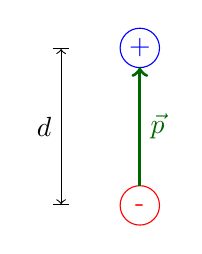
\begin{tikzpicture}
    \draw[blue] (0,1) circle (0.25cm) node {+};
    \draw[red] (0,-1) circle (0.25cm) node {-};
    \draw[|<->|] (-1,1) -- (-1,-1) node[pos=0.5,left] {\( d \)};
    \draw[->,black!60!green,very thick] (0,-0.75) -- (0,0.75)
      node[pos=0.5,right] {\( \vec{p} \)};
  \end{tikzpicture}
\end{center}
In this diagram, \( \vec{p} \) is the dipole moment. It points from negative to
positive and has a magnitude of \( qd \). For the on-axis field:
\[ \vec{E} = \frac{2k\vec{p}}{z^3} \quad \vec{p} = qd\j \]
For the off-axis field:
\[ \vec{E} = \frac{-k\vec{p}}{z^3} \quad \vec{p} = qd\j \]

\subsection*{Dipoles in Electric Fields}
\begin{center}
  \begin{tikzpicture}[scale=2]
    \node[black!60!green,right] at (4,2) {\( E \)};
    \foreach \y in {0,1,2} {
      \draw[->,black!60!green] (0,\y) -- (4,\y);
    }
    \draw[blue] (2,1.5) circle (0.1cm) node {+};
    \draw[red] (1,0.5) circle (0.1cm) node {-};
    \draw[dashed] (1.1,0.6) -- (1.9,1.4) node[pos=0.65,right] {\( \theta \)};
    \draw[|<->|] (0.75,0.75) -- (1.75,1.75) node[pos=0.5,above] {\( d \)};
  \end{tikzpicture}
\end{center}
\begin{align*}
  \vec{F} &= q\vec{E}+(-q\vec{E}) = 0 \\
  |\tau| &= dq\vec{E}\sin\theta = \vec{p}\vec{E}\sin\theta \\
  \tau &= \vec{p}\times\vec{E}
\end{align*}

\begin{center}
  You can find all my notes at \url{http://omgimanerd.tech/notes}. If you have
  any questions, comments, or concerns, please contact me at
  alvin@omgimanerd.tech
\end{center}

\end{document}
